\section{System and Correction Simulation}

\subsection{Modelling of Ground Effects}

This section describes how a realistic ground motion model was created using the power density spectrum and the correlation between the motion of each quadrupole. This part is mainly based on \cite{montag1999simulation}.

Disturbances in the electron beam can cause degradation in luminosity due to beam displacement at the iteration point and emittance growth. The motion of the quadrupoles depends strongly on the correlation length of the ground motion. Therefore, the ground vibration model has to take into account not only the motion at a single point, but also the coherence properties of the ground motion. In addition, the model has to consider the circular shape of the machine.

The power spectrum $P_{tot}(w)$ of ground motion at a single point can be approximate by:
\begin{align} 
    P_{tot}(w) = \frac{B}{w^4}
\end{align}
where $B$ is some proportionality constant characteristic of the site and $w = 2 \pi f$. It it shown an example in \ref{fig:power_spectrum}. According to the ATL rule, the power spectrum $\rho(w, L)$ of the uncorrelated motion of two points at a distance L is:
\begin{align} 
    \rho(w, L) = \frac{A L}{w^2}.
\end{align}
The uncorrelated part of motion must be smaller than the total motion, therefore
\begin{align} 
    \rho(w, L) \leq P_{tot}(w) \textrm{ for all } w.
\end{align} 

The coherent part of the motion of the ($n$ + 1)st magnet with respect to the $n$th is obtained with first order lowpass filter with cutoff frequency $w_0 = \sqrt{B/(A L)}$ is
\begin{align} 
    P_{corr, n+1}(w) = \bigg | \frac{w_0}{s + w_0} \bigg | ^2 P_{tot, n}(w) = \bigg | \frac{w_0}{s + w_0} \bigg | ^2 \frac{B}{w^4}.
\end{align}
And the uncorrelated motion obtained with a high pass filter with cutoff frequency of $w_0$ is
\begin{align} 
    P_{uncorr, n+1}(w) = \bigg | \frac{s}{s + w_0} \bigg | ^2 P_{n+1}(w).
\end{align}

To reflect the periodicity of the circular accelerator, it is necessary to correct the positions of all the magnets by 
\begin{align} 
   {y_n}^*(t) = y_n(t) - \frac{y_{N+1}(t) - y_1(t)}{L_{tot, N+1}}L_{tot, n}
\end{align}
where $L_{tot, n}$ is the total distance between 1st and the $n$th magnet

\begin{figure}
    \begin{center}
        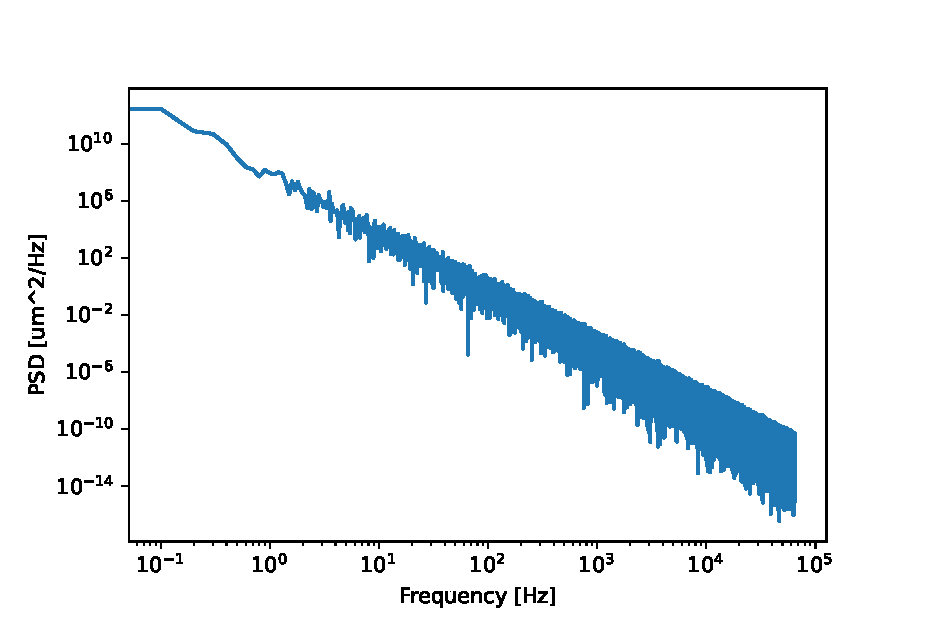
\includegraphics{power_spectrum.eps}
    \end{center}
    \caption{Simulated power spectrum at a single point.}
    \label{fig:power_spectrum}
\end{figure}

\subsection{Theorical Background}

\subsection{Simulation Model}

\subsection{Simulation Results}

\subsection{Robust Stability Analysis}

\subsection{pyAT}
